\documentclass[a4paper,11pt, twoside]{article}
\newcommand{\n}[1]{\textbf{#1}}
\usepackage{graphicx}
\usepackage{amsfonts}
\usepackage{amsmath}
\usepackage[brazilian]{babel}
\usepackage[utf8]{inputenc}
\usepackage[T1]{fontenc}
\usepackage {multirow}
\usepackage {booktabs}
\usepackage {fancyhdr}
\usepackage {graphicx}
\usepackage{xcolor}
\linespread {1.5}
\date{\today}
\author{Caio Vinícius Dadauto - 7994808}
\title{Exercicío de Programa 1}
\usepackage{listings}
\lstset{numbers=left,
stepnumber=1,
firstnumber=1,
numberstyle=\tiny,
extendedchars=false,
breaklines=flase,
tabsize=2,
showtabs=true,
tab=\textcolor{gray}{$\cdots$},
frame=tb,
basicstyle=\footnotesize,
stringstyle=\ttfamily,
showstringspaces=false}
\renewcommand{\lstlistingname}{Programa}
\renewcommand{\lstlistlistingname}{Lista de Listagens}
\begin{document}
    \pagestyle{fancy}
    \fancyhf{}
    \renewcommand{\footrulewidth}{0.1pt}
    \renewcommand{\headrulewidth}{0.0pt}
    \fancyfoot[LE, RO]{\bfseries \thepage}

    \begin{center}
        \begin{tabular}{c}
            {\huge Exercício de Programa 4}\\[-0.5cm]
            \rule{0.6\textwidth}{0.1mm}\\
            Caio Vinícius Dadauto$\quad$7994808\\
            {\small 16 de junho de 2013}
        \end{tabular}
    \end{center}
    \vspace{2cm}

    \section*{Problema I}
    A partir das condições iniciais $y(0) = 0$ e $\dot{y}(0) = 0$ e, ainda, da equação
    diferencial ordinaria de segunda ordem,
    \begin{eqnarray}\label{dif1}
        \dot{z} & = & \dot{y} - y + t^3 - 3t^2 + 6t\\
        z & = & \dot{y}
    \end{eqnarray}
    foram implementados dois programas com o intuito de determinar $y(5)$ e $\dot{y}(5)$.
    O primeiro programa aproxima tais valores aplicando o método de Euler, 
    o qual segue logo abaixo.
    {\linespread{1.15}
    \lstinputlisting[language=C, label=sqlselect, caption={Implementação 
    para o método de Euler.}]{euler.c}}
    
    Já o segundo programa aplica o método de Runge-Kutta clássico de quarta ordem que 
    segue abaixo.
    {\linespread{1.15}
    \lstinputlisting[language=C, label=sqlselect, caption={Implementação 
    para o método de Runge-Kutta.}]{RK4.c}}
    
    Os valores obtidos para $y(5)$ e $\dot{y}(5)$, a partir do método de Euler e do método de Runge-Kutta, são 
    apresentados a seguir:
    {\linespread{1}
    \begin{table}[!th]
        \begin{center}
            \begin{tabular}{ c c }
                \toprule[0.11em]
                \multirow{2}{*}{\n{Euler}} & \n{$y(5)$} = 125.565125\\
                & \n{$\dot{y}(5)$} = 75.914657\\
                \midrule
                \multirow{2}{*}{\n{Runge-Kutta}} & \n{$y(5)$} = 124.999999\\
                & \n{$\dot{y}(5)$} = 74.999999\\
                \toprule[0.11em]
            \end{tabular}
        \end{center}
    \end{table}}
    
    Como a solução da equação \eqref{dif1} é $y = t^3$, é claramente observavel (analisando os resultados acima)
    que o método de Runge-Kutta é muito mais acurado que o método de Euler, assim como era esperado.
    
    \section*{Problema II}
    \subsection*{Item 1}
    \subsubsection*{Item 1 - A}
    Para determinar o diagrama de fase ($\dot{x}\times x$)
    dado pela solução da equação do potencial de poço duplo,
    \begin{equation}\label{dif2}
        \ddot{x} - \frac{x}{2}(1 - x^2) = 0
    \end{equation}
    foi implementado um programa que aplica o método de Runge-Kutta de quarta ordem com um passo de 0.05.
    O qual é responsável por aproximar os pontos do plano $\dot{x}\times x$.
    
    O diagrama de fase foi plotado para três condições iniciais distintas de $\dot{x}(0)$ com $x(0) = -1$.
    Segue os diagramas obtido para cada uma das condições iniciais de $\dot{x}(0)$.
    \begin{figure}[!ht]
        \centering
        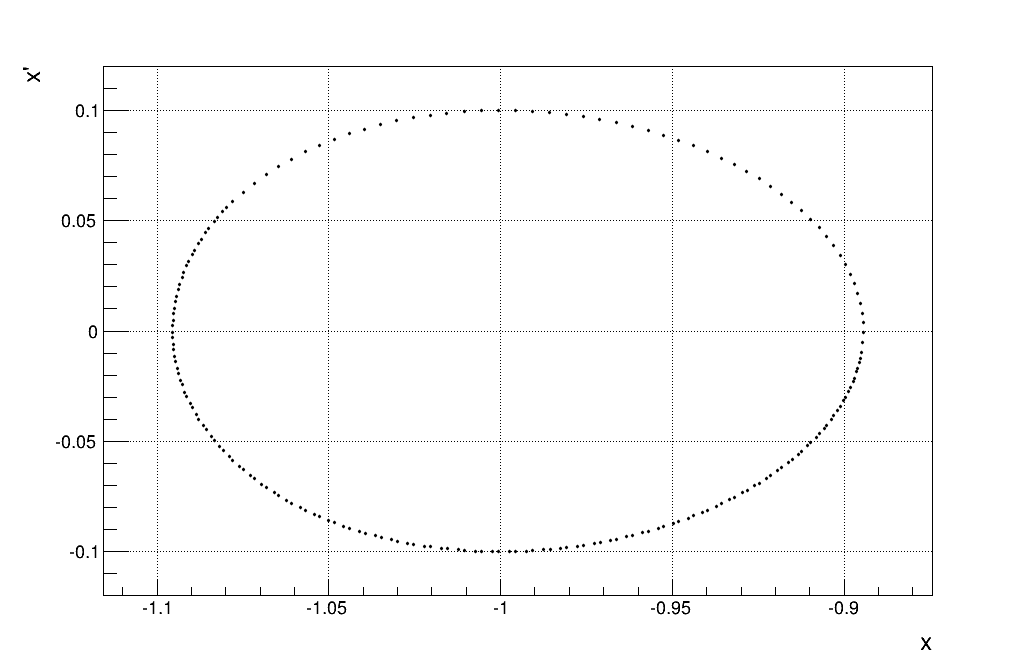
\includegraphics[scale=0.28]{poco01.png}
        \caption{Diagrama de fase para $\dot{x}(0) = 0.1$.\label{01}}
    \end{figure}
    \begin{figure}[!ht]
        \centering
        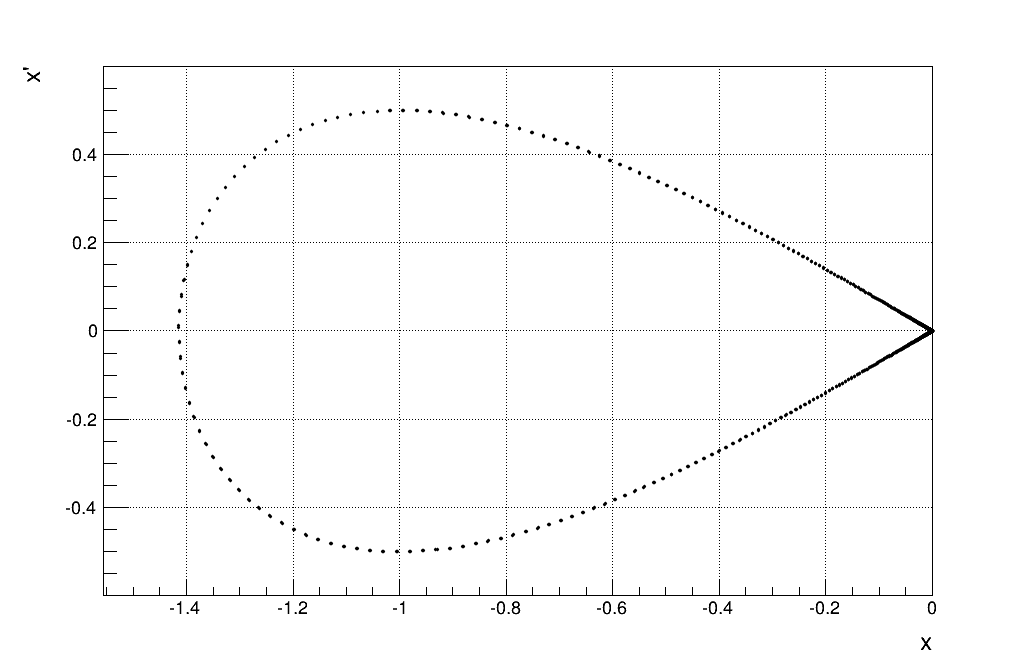
\includegraphics[scale=0.28]{poco05.png}
        \caption{Diagrama de fase para $\dot{x}(0) = 0.5$.\label{05}}
    \end{figure}
    \begin{figure}[!ht]
        \centering
        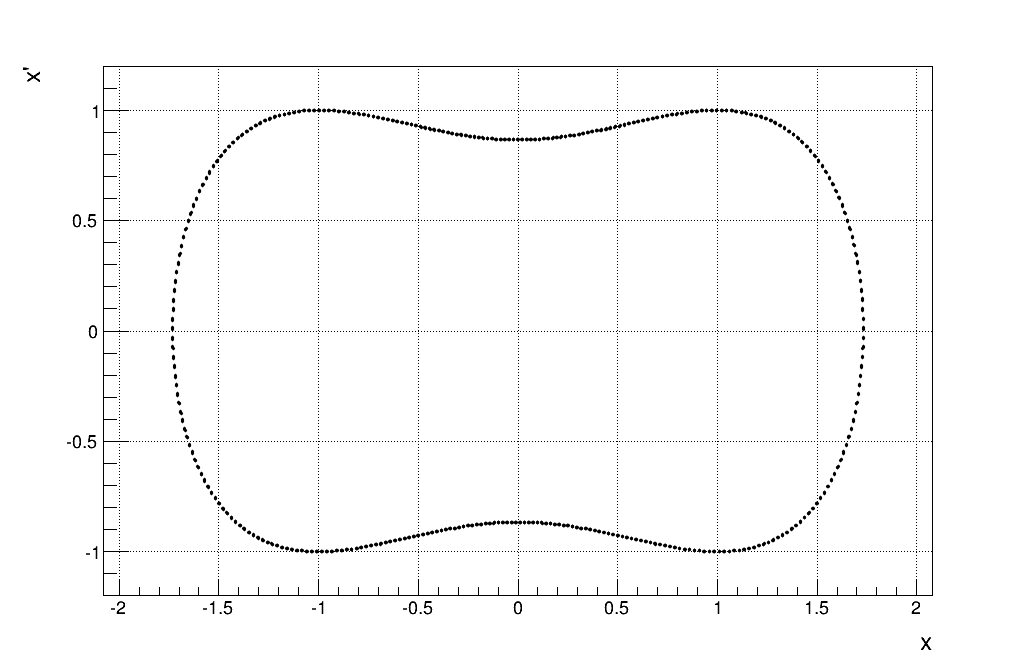
\includegraphics[scale=0.27]{poco1.png}
        \caption{Diagrama de fase para $\dot{x}(0) = 1$.\label{1}}
    \end{figure}
    
    \subsubsection*{Item 1 - B}
    Incluindo amortecimento a equeção \eqref{dif2}, tem-se:
    \begin{equation}\label{dif3}
        \ddot{x} + 2\gamma\dot{x} - \frac{x}{2}(1 - x^2) = 0
    \end{equation}
    Procedendo de forma semelhante ao item 1 - A, porém, agora, fixando $\dot{x}(0) = 1$
    e $x(0) = -1$, foram plotados dois diagramas de fase, cada qual para um valor distinto de
    $\gamma$. Diagramas, estes,  que seguem abaixo.
    \begin{figure}[!ht]
        \centering
        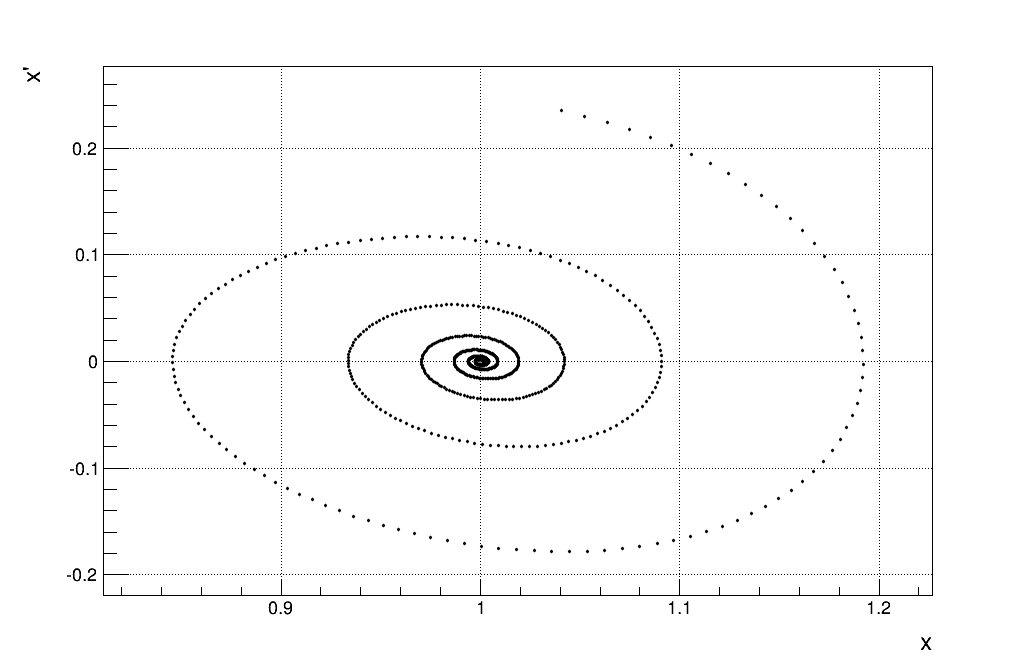
\includegraphics[scale=0.26]{amort025.png}
        \caption{Diagrama de fase para $\gamma = 0.125$.\label{025}}
    \end{figure}
    \begin{figure}[!ht]
        \centering
        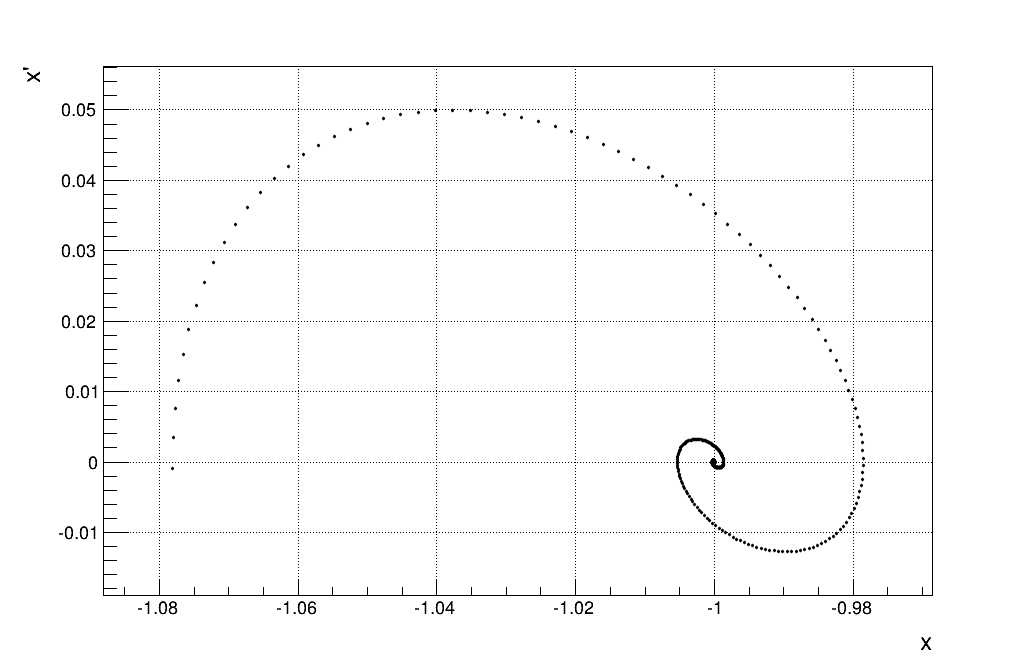
\includegraphics[scale=0.28]{amort08.png}
        \caption{Diagrama de fase para $\gamma = 0.4$.\label{08}}
    \end{figure}
    
    \subsubsection*{Item 1 - C}
    Forçando o sistema dado pela equação \eqref{dif3} com uma força $F$ de período $2\pi$, tem-se
    a seguinte equação:
    \begin{equation}\label{dif4}
        \ddot{x} + 0.25\dot{x} - \frac{x}{2}(1 - x^2) = F\cos{t}
    \end{equation}
    
    Tomando como condições iniciais $\dot{x}(0) = 1$ e $x(0) = -1$, foram
    plotados quatro diagramas de fase distintos, cada qual para um valor de F (0.22, 0.28, 0.35, 0.6).
    Ao plotar cada diagrama foram desconsiderados os primeiros 7000 pontos obtidos
    pela evolução do Runge-Kutta, com o intuito de eliminar o transiente.
    
    Como exemplo de programa, é apresentado abaixo o código implementado para plotar
    o diagrama de fase quando $F$ vale 0.6. Sendo que no programa para os demais diagramas ($F = 0.22$, $F = 0.28$, $F = 0.35$)
    foi modificado apenas o valor da força na função rotulada por ``funcao''.
    \newpage
    {\linespread{1.15}
    \lstinputlisting[language=C, label=sqlselect, caption={Implementação 
    para plotar o diagrama de fase da equação \eqref{dif4} quando $F = 0.6$.}]{forcado.c}}
    
    Segue os diagramas de fase obtidos para cada valor distinto de F.
    \begin{figure}[!ht]
        \centering
        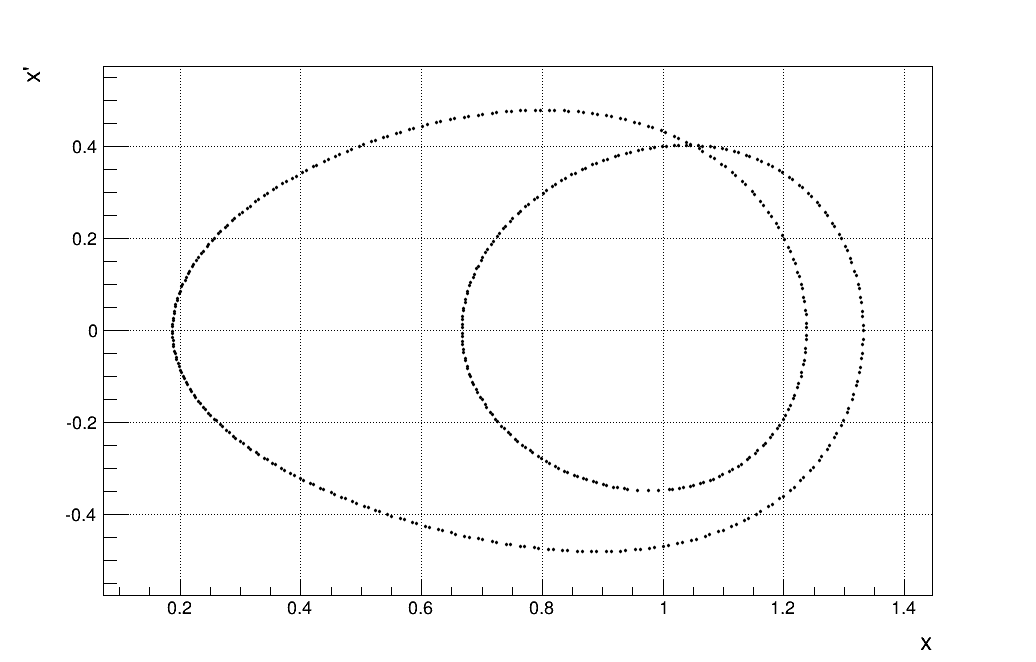
\includegraphics[scale=0.28]{forc022.png}
        \caption{Diagrama de fase para $F = 0.22$.\label{022}}
    \end{figure}
    \begin{figure}[!ht]
        \centering
        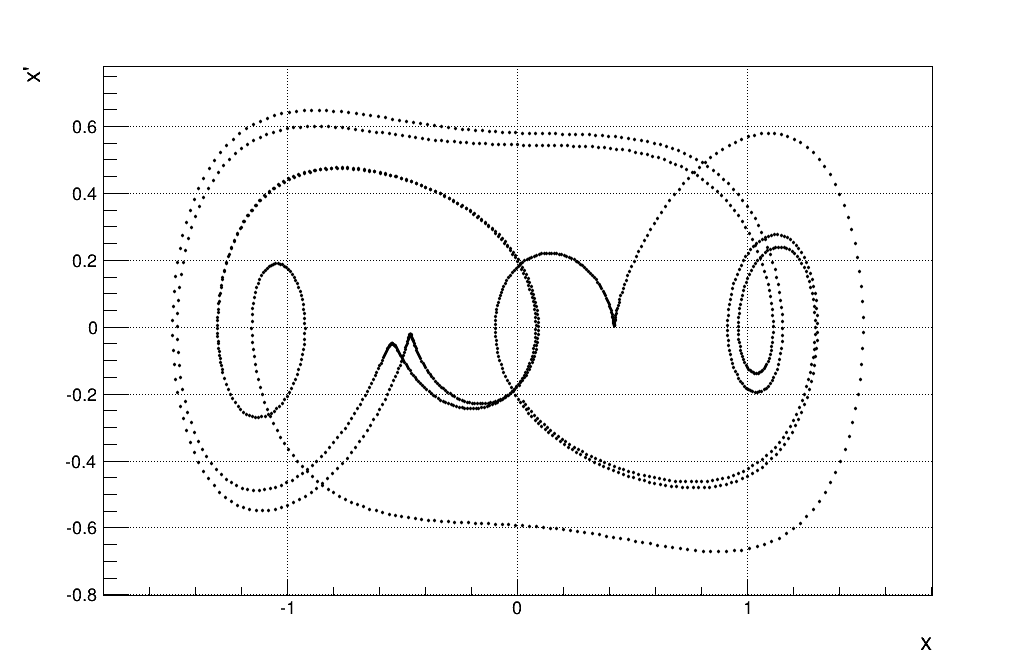
\includegraphics[scale=0.28]{forc028.png}
        \caption{Diagrama de fase para $F = 0.28$.\label{028}}
    \end{figure}
    \newpage
    \begin{figure}[!ht]
        \centering
        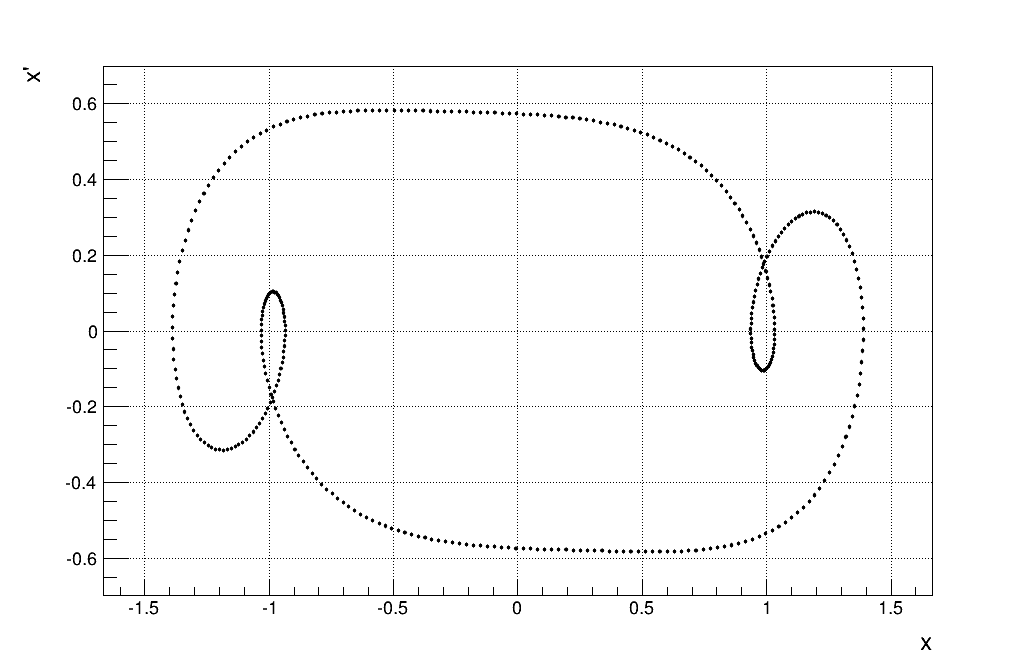
\includegraphics[scale=0.27]{forc035.png}
        \caption{Diagrama de fase para $F = 0.35$.\label{035}}
    \end{figure}
    \begin{figure}[!ht]
        \centering
        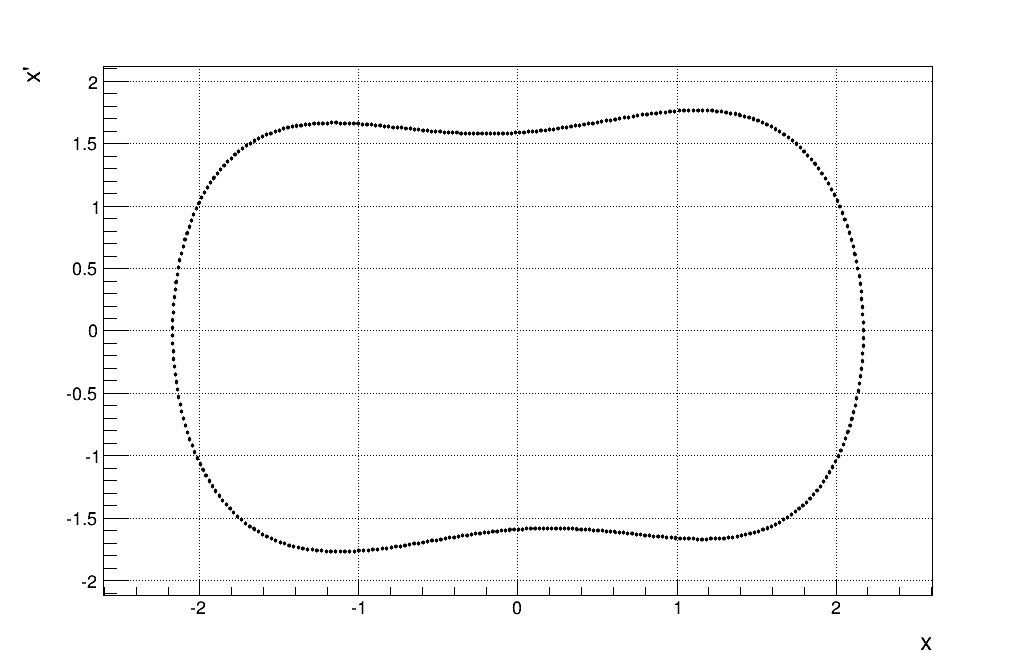
\includegraphics[scale=0.27]{forc06.png}
        \caption{Diagrama de fase para $F = 0.6$.\label{06}}
    \end{figure}
    
    No item 1 - A os atratores são dados pelas curvas definidas
    nos diagramas de fase das figuras \ref{01}, \ref{05} e \ref{1}.
    No item 1 -B os atratores  são os pontos, no plano $\dot{x}\times x$, (1; 0) e (-1; 0) 
    para $\gamma = 0.125$ e para $\gamma = 0.4$, respectivamente.
    Por fim, no item 1 - C os atratores, para  $F = 0.22$, $F = 0.35$ e $F = 0.6$,
    são dados pelas curvas definidas
    nos diagramas de fase das figuras \ref{022}, \ref{035} e \ref{06}. Contudo,
    para $F = 0.28$ o atrator é caótico como se pode observar na figura \ref{028}.
    
    \subsection*{Item 2}
    Partindo da equação \eqref{dif4} e das mesmas condições iniciais do item 1 - C é possível
    plotar um diagrama de bifurcação. Bastando para isso plotar sussecivas secções de Poincaré
    a cada período do elemento forçador F (que nesse caso é $2\pi$) para um numero discreto de 
    valores de $F$ dentro de um intervalo.
    
    Assim, foi implementado um programa que toma $[0; 0.7]$ como o intervalo de $F$, o qual progride 
    em passos de 0.0005 de forma a discretizar o intervalo. A cada valor de $F$ são plotadas 100 secções de
    Poincaré por periodo de $F$. O tempo $t$, por sua vez, varia de 0 a $2\pi$ (período de $F$) em passos de 0.002$\pi$
    de forma que para se completar um periodo seja necessario 1000 interações de Runge-Kutta.
    É ainda relalizada 200000 interações de Runge-Kutta a cada novo valor de 
    $F$ de forma a eliminar a região de transiente.
    Tal programa segue logo abaixo.
    
    {\linespread{1.15}
    \lstinputlisting[language=C, label=sqlselect, caption={Implementação 
    para plotar o diagrama de fase para a equação \eqref{dif4}.}]{cte.c}}
    \newpage
    A partir do programa acima, obteve-se o diagrama de bifurcação apresentado na figura \ref{bifur}.
    \begin{figure}[!ht]
        \centering
        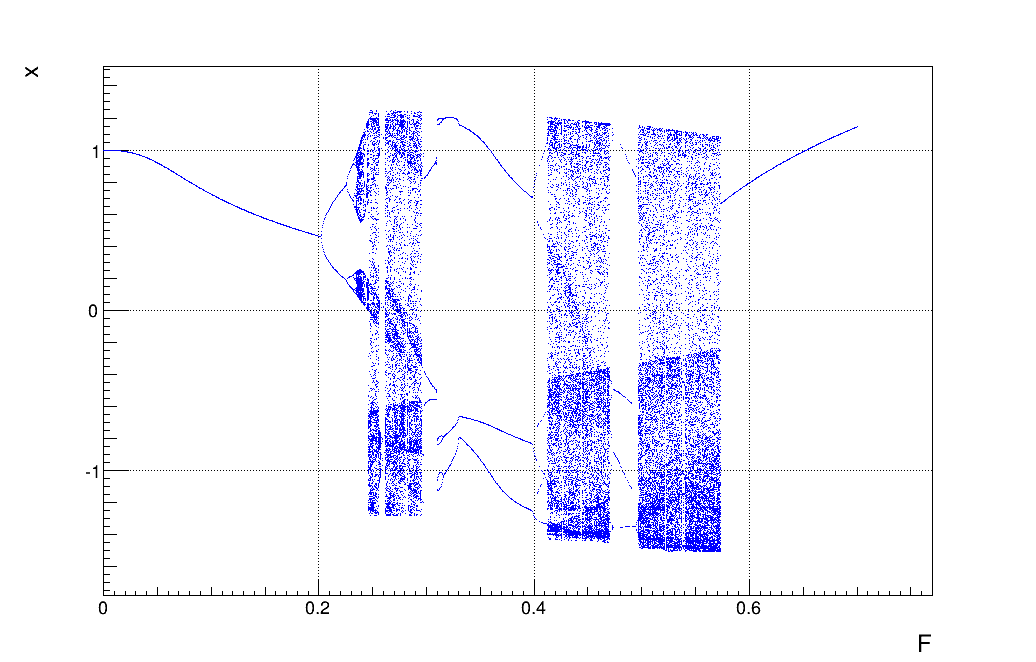
\includegraphics[scale=0.4]{bifur.png}
        \caption{Diagrama de bifurcação para a equação \eqref{dif4}.\label{bifur}}
    \end{figure}
    
    Com o objetivo de determinar a constante de Feigenbaum ($\delta$) a figura \ref{bifur} foi ampliada
    de forma a analisar o intervalo $[0.232; 0.234]$ de $F$ e o intervalo $[0.2; 0.25]$ de $X$, tal ampliação 
    é apresentada na figura \ref{bifur-amp}. Nesta figura são indicados dois intervalos ($\Delta_1$ e $\Delta_2$),
    que correspondem a variação de $F$ em duas bifurcações concecutivas. Assim, tem-se que a constante de
    Feigenbaum é dada, aproximadamente, por:
    \begin{equation}\label{feig}
        \delta = \frac{\Delta_1}{\Delta_2}
    \end{equation}

    A partir da leitura do gráfico apresentado na figura \ref{bifur-amp} é possível 
    determinado o valor de $\Delta_1 = 1.64\cdot 10^{-3}$ e $\Delta_2 = 3.8\cdot 10^{-4}$.
    Portanto, partindo da equação \eqref{feig}, tem-se que:
    \begin{displaymath}
        \delta = 4.31579
    \end{displaymath}
    \begin{figure}[!ht]
        \centering
        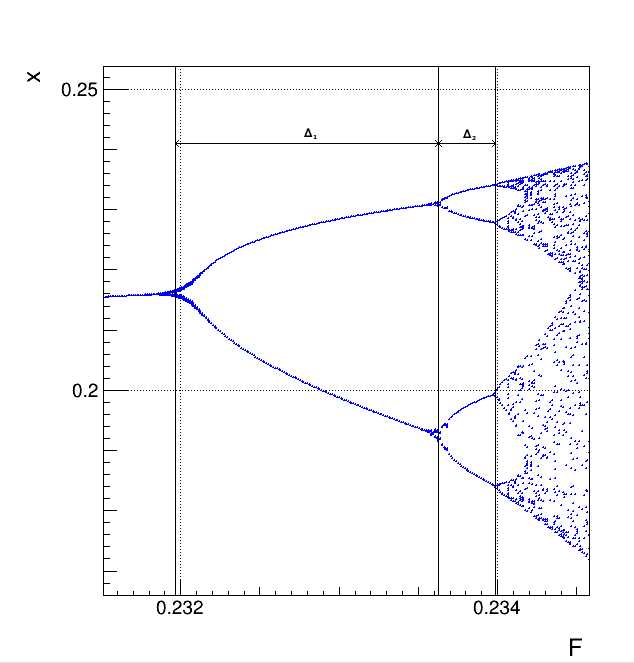
\includegraphics[scale=0.4]{bifur1.png}
        \caption{Ampliação do diagrama de bifurcação apresentado na figura \ref{bifur}.\label{bifur-amp}}
    \end{figure}
    
    \section*{Problema II}
    Para $F$ constante, igual a 0.27, e nas mesmas condições iniciais do item 2,
    é possível sobrepor 2000 secções de Poincaré, onde cada secção é tomada
    após um ciclo do elemento forçador $F$.
    
    De forma semelhante ao item 2, foram realizadas inicialmente 
    200000 interações de Runge-Kutta com o intuito de eleminar o transiente.
    A sobreposição de 2000 secções de Poincaré é apresentada na figura \ref{poin}.
    \newpage
    \begin{figure}[!ht]
        \centering
        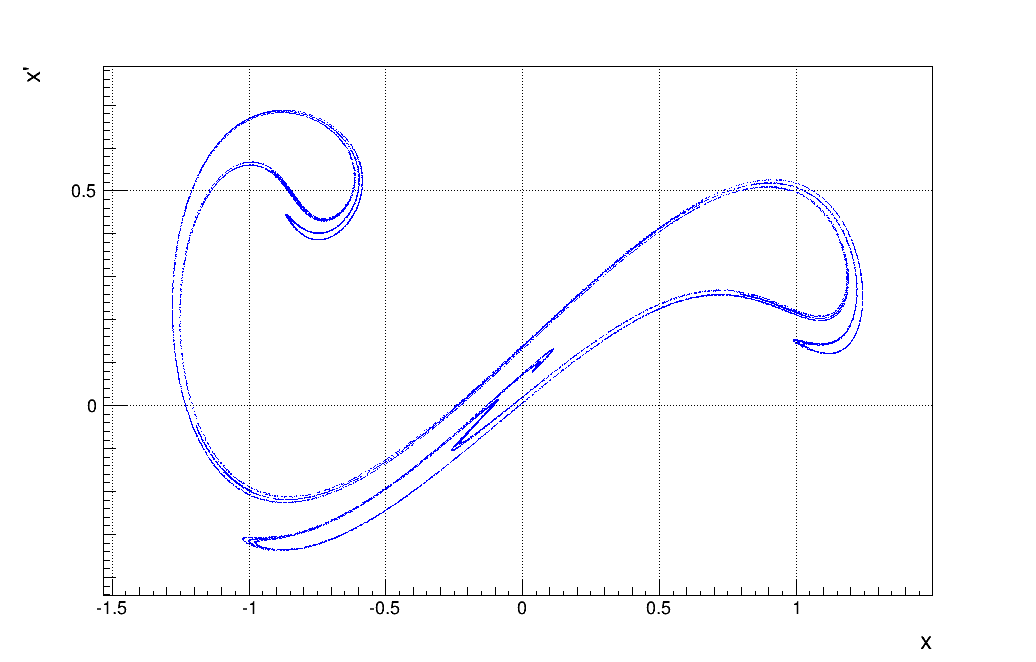
\includegraphics[scale=0.35]{pan.png}
        \caption{Sobreposição de 2000 secções de Poincaré.\label{poin}}
    \end{figure}
    
    
\end{document}